\documentclass[letterpaper, 11pt]{article}
% load packages
\usepackage[utf8]{inputenc}
\usepackage{amsmath}
\usepackage{amssymb}
\usepackage{amsthm}
\usepackage{mathtools}
\usepackage[margin=0.5in]{geometry} 
\usepackage{graphicx}
\usepackage{color}
\usepackage{physics}
\usepackage{comment}
%outline packages
\usepackage{outlines}
\usepackage{enumitem}
\usepackage{setspace}

% set up the outline stuff-----------------
\newcommand{\ItemSpace}{0pt}
\newcommand{\ParSpace}{-0pt}
%\setlist[enumerate]{itemsep=0pt}
\setenumerate[1]{itemsep={\ItemSpace},parsep={\ParSpace},label=\textbf{\large \Roman*.}}
\setenumerate[2]{itemsep={\ItemSpace},parsep={\ParSpace},label=\textbf{\Alph*.} }
\setenumerate[3]{itemsep={\ItemSpace},parsep={\ParSpace},label=\roman*.}
\setenumerate[4]{itemsep={\ItemSpace},parsep={\ParSpace},label=\alph*.}
%define the style of outline  ----------
\newcommand{\lb}[1]{\textbf{ \large #1 } }
%end definitions of outline ------------

% pictures. 
\usepackage{tikz} 
\usepackage{circuitikz}
\usetikzlibrary{calc}
\usepackage{pgfplots}
\pgfplotsset{compat=1.12} % for filldraw points..

% use multi column
\usepackage{multicol} 

% rewrite definitions
\renewcommand{\Re}{\rm{Re}}
\renewcommand{\Im}{\rm{Im}}
\renewcommand{\imath}{\rm{i}}
\renewcommand{\rm}{\mathrm}
\renewcommand{\le}{\left<}
%new commands
\newcommand{\ri}{\right>}
\newcommand{\euler}{\rm{e}}
%for expect and correlated parts 
\newcommand{\cor}[1]{\Delta \left< #1 \right> }
\newcommand{\expect}[1] {\left< #1 \right> } 
\begin{document} 
\begin{flushright} \noindent\today \end{flushright} 

\noindent 
%------------------------------------
{ \bf \Large Problems } \\ 
%------------------------------------
 

\noindent { \bf U00T01T01: } Simplify the fractions.   \\ 
\begin{multicols}{ 3 }
\noindent { \bf  Problem 01: }
\begin{align} 
\frac{ 9k / 3p  } { 5q / 3c  }  \nonumber 
\end{align} 
\noindent { \bf  Problem 02: }
\begin{align} 
\frac{ t / 5w  } { 10w / 10r  }  \nonumber 
\end{align} 
\end{multicols}

\noindent { \bf U00T02T01: } Solve for $x$.  \\ 
\begin{multicols}{ 3 }
\noindent { \bf  Problem 03: }
\begin{align} 
\frac{  -5f }{   -5z  } = \frac {  -7s }{ x  }  \nonumber 
\end{align} 
\noindent { \bf  Problem 04: }
\begin{align} 
\frac{  -p }{  8y  } = \frac { x }{  -9u  }  \nonumber 
\end{align} 
\end{multicols}

\noindent { \bf U00T02T02: } Solve for $x$  \\ 
\begin{multicols}{ 2 }
\noindent { \bf  Problem 05: }
\begin{align} 
 -3gx +20u &= 18l \nonumber 
\end{align} 
\noindent { \bf  Problem 06: }
\begin{align} 
 -5wx +20b &=  -17l \nonumber 
\end{align} 
\end{multicols}

\noindent { \bf U01T01T01: } Find the x- and y-components given the magnitude and direction of the vector.  \\ 
\begin{multicols}{ 2 }
\noindent { \bf  Problem 07: }
\begin{align}  
A =  7.81, \theta =  0.78 \pi \nonumber   
\end{align}    
\noindent { \bf  Problem 08: }
\begin{align}  
A =  8.25, \theta =  1.42 \pi \nonumber   
\end{align}    
\end{multicols}

\noindent { \bf U01T01T02: } Find the magnitude and remaining component, given the angle and a component.  \\ 
\begin{multicols}{ 2 }
\noindent { \bf  Problem 09: }
\begin{align}  
A_x &=  8.00 \nonumber  
\end{align}   
\hspace{3cm} $ \theta = $  0.04 $\pi$ 
\noindent { \bf  Problem 10: }
\begin{align}  
A_y &=  4.00 \nonumber  
\end{align}   
\hspace{3cm} $ \theta = $  0.87 $\pi$ 
\end{multicols}

\noindent { \bf U01T01T03: } Given the vector components, find the magnitude and direction. Specify angle in terms of cardinal directions, e.g. 30 degree north of east.  \\ 
\begin{multicols}{ 2 }
\noindent { \bf  Problem 11: }
\begin{align}  
A_x =  8.00 \nonumber \\  
A_y =  9.00 \nonumber
\end{align}   
\noindent { \bf  Problem 12: }
\begin{align}  
A_x = -6.00 \nonumber \\  
A_y = -1.00 \nonumber
\end{align}   
\end{multicols}

\noindent { \bf U01T02T01: } Add the two vectors.  \\ 
\begin{multicols}{ 2 }
\noindent { \bf  Problem 13: }\begin{align}
A &=  9.49 \nonumber \\
\theta_A &=  0.60 \pi \nonumber \\
B &=  9.49 \nonumber \\
\theta_B &=  0.60 \pi \nonumber \\
\nonumber \end{align}\noindent { \bf  Problem 14: }\begin{align}
A &=  2.83 \nonumber \\
\theta_A &=  0.25 \pi \nonumber \\
B &=  2.83 \nonumber \\
\theta_B &=  0.25 \pi \nonumber \\
\nonumber \end{align}\end{multicols}

\noindent { \bf U01T02T02: } Add the three vectors.  \\ 
\begin{multicols}{ 2 }
\noindent { \bf  Problem 15: }\begin{align}
A &=  8.60 \nonumber \\
\theta_A &=  0.80 \pi \nonumber \\
B_x &= -7.00 \nonumber \\  
B_y &=  5.00 \nonumber \\
C_x &= -7.00 \nonumber \\  
C_y &=  5.00 \nonumber \\
\nonumber \end{align}\noindent { \bf  Problem 16: }\begin{align}
A &= 12.73 \nonumber \\
\theta_A &=  0.25 \pi \nonumber \\
B_x &=  9.00 \nonumber \\  
B_y &=  9.00 \nonumber \\
C_x &=  9.00 \nonumber \\  
C_y &=  9.00 \nonumber \\
\nonumber \end{align}\end{multicols}

\noindent { \bf U01T02T03: } Add the four vectors.  \\ 
\noindent { \bf  Problem 17: }\begin{align}
A &=  7.00 \nonumber \\
\theta_A &=  1.00 \pi \nonumber \\
B &=  7.00 \nonumber \\
\theta_B &=  1.00 \pi \nonumber \\
C &=  7.00 \nonumber \\
\theta_C &=  1.00 \pi \nonumber \\
D_x &= -7.00 \nonumber \\  
D_y &=  0.00 \nonumber \\
\nonumber \end{align}\noindent { \bf  Problem 18: }\begin{align}
A_x &= -3.00 \nonumber \\  
A_y &= -8.00 \nonumber \\
B_x &= -3.00 \nonumber \\  
B_y &= -8.00 \nonumber \\
C &=  8.54 \nonumber \\
\theta_C &=  1.39 \pi \nonumber \\
D_x &= -3.00 \nonumber \\  
D_y &= -8.00 \nonumber \\
\nonumber \end{align}

\pagebreak 
%------------------------------------
{ \bf \Large Solutions } \\ 
%------------------------------------
 

\noindent { \bf U00T01T01: } 
Multiple the top fraction by the reciprocal, i.e. 
\begin{align}
\frac{ a / b } { c / d } &= \left( \frac{a}{b}  \right)  \left( \frac{d}{c} \right)  = \frac{ a d } { b c }  \nonumber 
\end{align} 
 \\ 
\begin{multicols}{ 3 }
\noindent { \bf  Problem 01: } 
\begin{align} 
\frac{ 9ck  } { 5pq  }  \nonumber 
\end{align} 
\noindent { \bf  Problem 02: } 
\begin{align} 
\frac{ rt  } { 5w^2  }  \nonumber 
\end{align} 
\end{multicols}

\noindent { \bf U00T02T01: } Cross multiply and then simplify. \\ 
\begin{multicols}{ 3 }
\noindent { \bf  Problem 03: } 
\begin{align} 
 -5fx &= 35sz \implies x = \frac{ 7sz } {  -f }   \nonumber  
\end{align} 
\noindent { \bf  Problem 04: } 
\begin{align} 
9pu &= 8xy \implies x = \frac{ 9pu } { 8y }   \nonumber  
\end{align} 
\end{multicols}

\noindent { \bf U00T02T02: } Isolate $x$ by first subtracting and then dividing by coefficient of $x$. \\ 
\begin{multicols}{ 2 }
\noindent { \bf  Problem 05: } 
\begin{align} 
 -3gx &= 18l -20u \implies x = \frac{ 18l -20u } {  -3g }   \nonumber  
\end{align} 
\noindent { \bf  Problem 06: } 
\begin{align} 
 -5wx &=  -17l -20b \implies x = \frac{ 17l +20b } { 5w }   \nonumber  
\end{align} 
\end{multicols}

\noindent { \bf U01T01T01: } 
Assuming standard convention for the angle $[0,2\pi]$, the components of vector $\vec{A}$ can be found by
\begin{align}  
A_x &= A \cos (\theta)  \nonumber \\  
A_y &= A \sin (\theta)  \nonumber  
\end{align}  
 \\ 
\begin{multicols}{ 2 }
\noindent { \bf  Problem 07: } 
\begin{align}  
A_x &= A \cos (\theta) = -6.00 \nonumber \\  
A_y &= A \sin (\theta) =  5.00 \nonumber  
\end{align}  
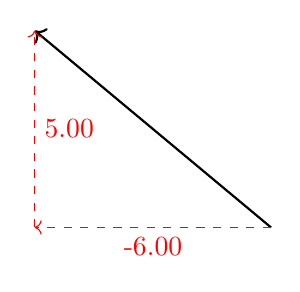
\begin{tikzpicture}[scale=0.5] 
\draw[->,black, thick] ( 0.00, 0.00) -- (-6.00, 5.00) node[midway,above,sloped]{  } ;
\draw[->,red,dashed] ( 0.00, 0.00) -- (-6.00, 0.00) node[midway,below]{ -6.00 };\draw[->,red,dashed] (-6.00, 0.00) -- (-6.00, 5.00) node[midway,right]{  5.00 }; 
\end{tikzpicture} \\
\noindent { \bf  Problem 08: } 
\begin{align}  
A_x &= A \cos (\theta) = -2.00 \nonumber \\  
A_y &= A \sin (\theta) = -8.00 \nonumber  
\end{align}  
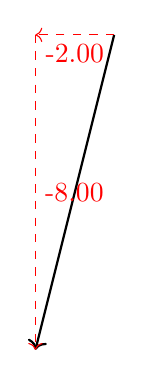
\begin{tikzpicture}[scale=0.5] 
\draw[->,black, thick] ( 0.00, 0.00) -- (-2.00,-8.00) node[midway,above,sloped]{  } ;
\draw[->,red,dashed] ( 0.00, 0.00) -- (-2.00, 0.00) node[midway,below]{ -2.00 };\draw[->,red,dashed] (-2.00, 0.00) -- (-2.00,-8.00) node[midway,right]{ -8.00 }; 
\end{tikzpicture} \\
\end{multicols}

\noindent { \bf U01T01T02: } 
Assuming standard convention for the angle $[0,2\pi]$, the components of vector $\vec{A}$ can be found by
\begin{align}  
A_x &= A \cos (\theta)  \nonumber \\  
A_y &= A \sin (\theta)  \nonumber  
\end{align}  
So this means that 
\begin{align}
A &= \frac{ A_x }{ \cos \theta } = \frac{ A_y }{ \sin \theta } \nonumber  \\
A_x &= \sqrt{ A^2 - A_y^2 } \nonumber \\
A_y &= \sqrt{ A^2 - A_x^2 } \nonumber 
\end{align} 
as the case may be. 
 \\ 
\begin{multicols}{ 2 }
\noindent { \bf  Problem 09: } 
\begin{align}  
 A &= A_x /  \cos (\theta)  =  8.06 \nonumber \\  
A_y &= \sqrt{ A^2 - A_x^2 }  =  1.00 \nonumber
\end{align}  
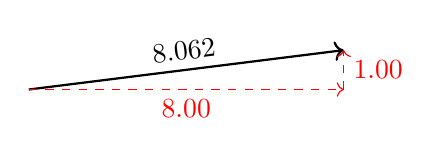
\begin{tikzpicture}[scale=0.5] 
\draw[->,black, thick] ( 0.00, 0.00) -- ( 8.00, 1.00) node[midway,above,sloped]{ 8.062 } ;
\draw[->,red,dashed] ( 0.00, 0.00) -- ( 8.00, 0.00) node[midway,below]{  8.00 };\draw[->,red,dashed] ( 8.00, 0.00) -- ( 8.00, 1.00) node[midway,right]{  1.00 }; 
\end{tikzpicture} \\
\noindent { \bf  Problem 10: } 
\begin{align}  
 A &= A_y /  \sin (\theta)  =  9.85 \nonumber \\  
 A_x &= \sqrt{ A^2 - A_y^2 }  = -9.00 \nonumber
\end{align}  
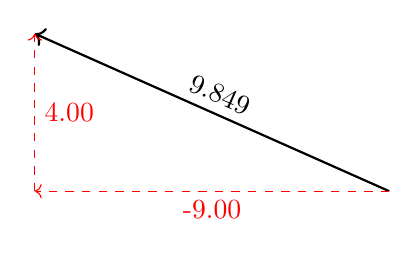
\begin{tikzpicture}[scale=0.5] 
\draw[->,black, thick] ( 0.00, 0.00) -- (-9.00, 4.00) node[midway,above,sloped]{ 9.849 } ;
\draw[->,red,dashed] ( 0.00, 0.00) -- (-9.00, 0.00) node[midway,below]{ -9.00 };\draw[->,red,dashed] (-9.00, 0.00) -- (-9.00, 4.00) node[midway,right]{  4.00 }; 
\end{tikzpicture} \\
\end{multicols}

\noindent { \bf U01T01T03: } 
Assuming standard convention for the angle $[0,2\pi]$, the components of vector $\vec{A}$ can be found by
\begin{align}  
A_x &= A \cos (\theta)  \nonumber \\  
A_y &= A \sin (\theta)  \nonumber  
\end{align}  
So this means that 
\begin{align}
A &= \sqrt{{ A_x^2 + A_y^2 }} \nonumber  \\
\tan \theta = \frac{{A_y}}{{A_x}} .  \nonumber 
\end{align} 
With the signs of the components you get the correct angle from $[0,2\pi)$. Then convert that to cardinal directions.   
 \\ 
\begin{multicols}{ 2 }
\noindent { \bf  Problem 11: } 
\begin{align}  
A = 12.04 \nonumber 
\end{align}  
\hspace{3cm} The direction is 48.366 degrees north of east . \\
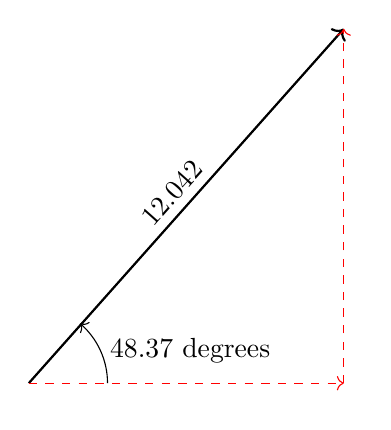
\begin{tikzpicture}[scale=0.5] 
\draw[->,black, thick] ( 0.00, 0.00) -- ( 8.00, 9.00) node[midway,above,sloped]{ 12.042 } ;
\draw[->,red,dashed] ( 0.00, 0.00) -- ( 8.00, 0.00) node[midway,below]{  };\draw[->,red,dashed] ( 8.00, 0.00) -- ( 8.00, 9.00) node[midway,right]{  }; 
\draw[->,black] ( 2.00, 0.00) arc (0:49.37: 2.00) node[midway,anchor=west] {  48.37 degrees } ;
\end{tikzpicture} \\
\noindent { \bf  Problem 12: } 
\begin{align}  
A =  6.08 \nonumber 
\end{align}  
\hspace{3cm} The direction is 9.462 degrees south of west . \\
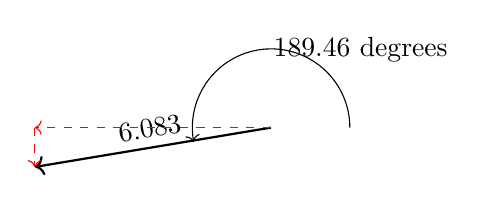
\begin{tikzpicture}[scale=0.5] 
\draw[->,black, thick] ( 0.00, 0.00) -- (-6.00,-1.00) node[midway,above,sloped]{ 6.083 } ;
\draw[->,red,dashed] ( 0.00, 0.00) -- (-6.00, 0.00) node[midway,below]{  };\draw[->,red,dashed] (-6.00, 0.00) -- (-6.00,-1.00) node[midway,right]{  }; 
\draw[->,black] ( 2.00, 0.00) arc (0:190.46: 2.00) node[midway,anchor=west] { 189.46 degrees } ;
\end{tikzpicture} \\
\end{multicols}

\noindent { \bf U01T02T01: } 
Assuming standard convention for the angle $[0,2\pi]$, the components of vector $\vec{A}$ can be found by
\begin{align}  
A_x &= A \cos (\theta)  \nonumber \\  
A_y &= A \sin (\theta)  \nonumber  
\end{align}  
We get the sum of a vector by adding together the components as 
\begin{align}
\vec{A} + \vec{B} &= \begin{pmatrix}
A_x + B_x \\ A_y + B_y   
\end{pmatrix} , \nonumber  
\end{align} 
for the number of vectors we have. 
 \\ 
\begin{multicols}{ 2 }
\noindent { \bf  Problem 13: } 
\begin{align}  
R_x &=  3.00 \nonumber \\  
R_y &= 11.00 \nonumber  
\end{align}  
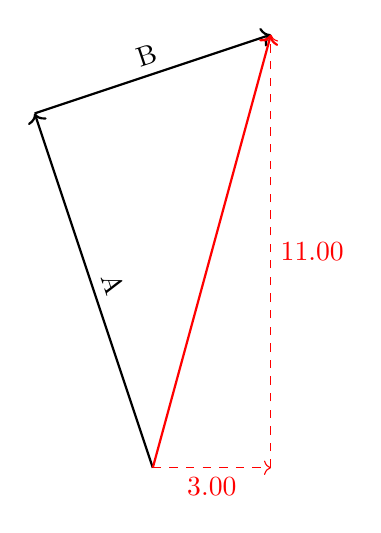
\begin{tikzpicture}[scale=0.5] 
\draw[->,black, thick] ( 0.00, 0.00) -- (-3.00, 9.00) node[midway,above,sloped]{ A } ;\draw[->,black, thick] (-3.00, 9.00) -- ( 3.00,11.00) node[midway,above,sloped]{ B } ;
\draw[->,red, thick] ( 0.00, 0.00) -- ( 3.00,11.00) node[midway,above,sloped]{  } ;
\draw[->,red,dashed] ( 0.00, 0.00) -- ( 3.00, 0.00) node[midway,below]{  3.00 };\draw[->,red,dashed] ( 3.00, 0.00) -- ( 3.00,11.00) node[midway,right]{ 11.00 }; 
\end{tikzpicture} \\
\noindent { \bf  Problem 14: } 
\begin{align}  
R_x &=  4.00 \nonumber \\  
R_y &= -8.00 \nonumber  
\end{align}  
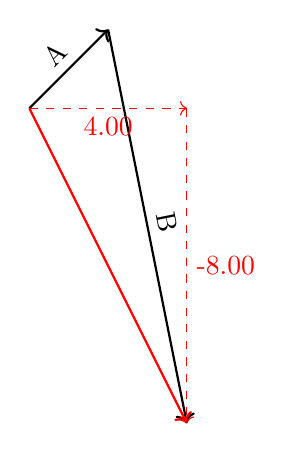
\begin{tikzpicture}[scale=0.5] 
\draw[->,black, thick] ( 0.00, 0.00) -- ( 2.00, 2.00) node[midway,above,sloped]{ A } ;\draw[->,black, thick] ( 2.00, 2.00) -- ( 4.00,-8.00) node[midway,above,sloped]{ B } ;
\draw[->,red, thick] ( 0.00, 0.00) -- ( 4.00,-8.00) node[midway,above,sloped]{  } ;
\draw[->,red,dashed] ( 0.00, 0.00) -- ( 4.00, 0.00) node[midway,below]{  4.00 };\draw[->,red,dashed] ( 4.00, 0.00) -- ( 4.00,-8.00) node[midway,right]{ -8.00 }; 
\end{tikzpicture} \\
\end{multicols}

\noindent { \bf U01T02T02: } 
Assuming standard convention for the angle $[0,2\pi]$, the components of vector $\vec{A}$ can be found by
\begin{align}  
A_x &= A \cos (\theta)  \nonumber \\  
A_y &= A \sin (\theta)  \nonumber  
\end{align}  
We get the sum of a vector by adding together the components as 
\begin{align}
\vec{A} + \vec{B} &= \begin{pmatrix}
A_x + B_x \\ A_y + B_y   
\end{pmatrix} , \nonumber  
\end{align} 
for the number of vectors we have. 
 \\ 
\begin{multicols}{ 2 }
\noindent { \bf  Problem 15: } 
\begin{align}  
R_x &= -15.00 \nonumber \\  
R_y &= 11.00 \nonumber  
\end{align}  
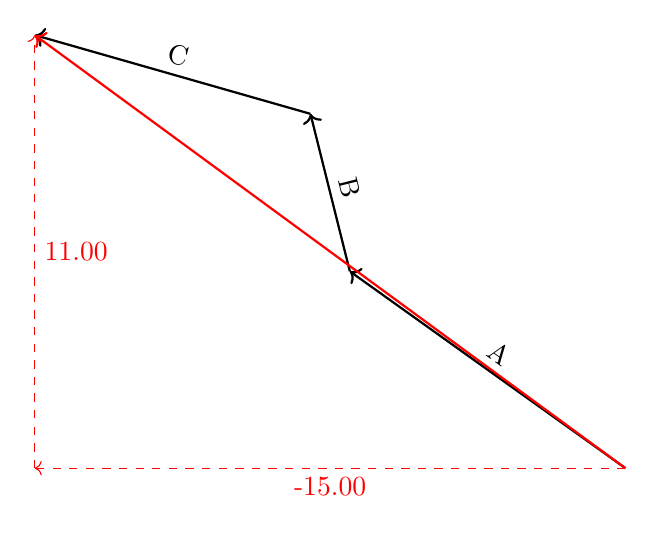
\begin{tikzpicture}[scale=0.5] 
\draw[->,black, thick] ( 0.00, 0.00) -- (-7.00, 5.00) node[midway,above,sloped]{ A } ;\draw[->,black, thick] (-7.00, 5.00) -- (-8.00, 9.00) node[midway,above,sloped]{ B } ;\draw[->,black, thick] (-8.00, 9.00) -- (-15.00,11.00) node[midway,above,sloped]{ C } ;
\draw[->,red, thick] ( 0.00, 0.00) -- (-15.00,11.00) node[midway,above,sloped]{  } ;
\draw[->,red,dashed] ( 0.00, 0.00) -- (-15.00, 0.00) node[midway,below]{ -15.00 };\draw[->,red,dashed] (-15.00, 0.00) -- (-15.00,11.00) node[midway,right]{ 11.00 }; 
\end{tikzpicture} \\
\noindent { \bf  Problem 16: } 
\begin{align}  
R_x &=  9.00 \nonumber \\  
R_y &= 12.00 \nonumber  
\end{align}  
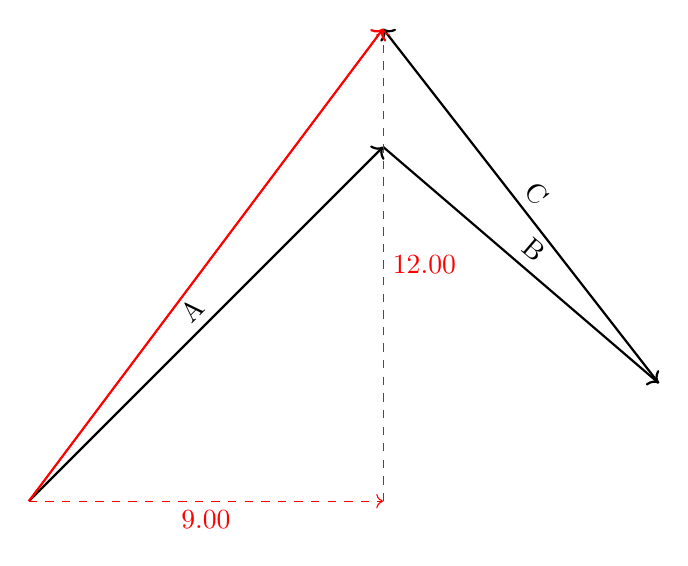
\begin{tikzpicture}[scale=0.5] 
\draw[->,black, thick] ( 0.00, 0.00) -- ( 9.00, 9.00) node[midway,above,sloped]{ A } ;\draw[->,black, thick] ( 9.00, 9.00) -- (16.00, 3.00) node[midway,above,sloped]{ B } ;\draw[->,black, thick] (16.00, 3.00) -- ( 9.00,12.00) node[midway,above,sloped]{ C } ;
\draw[->,red, thick] ( 0.00, 0.00) -- ( 9.00,12.00) node[midway,above,sloped]{  } ;
\draw[->,red,dashed] ( 0.00, 0.00) -- ( 9.00, 0.00) node[midway,below]{  9.00 };\draw[->,red,dashed] ( 9.00, 0.00) -- ( 9.00,12.00) node[midway,right]{ 12.00 }; 
\end{tikzpicture} \\
\end{multicols}

\noindent { \bf U01T02T03: } 
Assuming standard convention for the angle $[0,2\pi]$, the components of vector $\vec{A}$ can be found by
\begin{align}  
A_x &= A \cos (\theta)  \nonumber \\  
A_y &= A \sin (\theta)  \nonumber  
\end{align}  
We get the sum of a vector by adding together the components as 
\begin{align}
\vec{A} + \vec{B} &= \begin{pmatrix}
A_x + B_x \\ A_y + B_y   
\end{pmatrix} , \nonumber  
\end{align} 
for the number of vectors we have. 
 \\ 
\noindent { \bf  Problem 17: } 
\begin{align}  
R_x &= -7.00 \nonumber \\  
R_y &= 15.00 \nonumber  
\end{align}  
\begin{tikzpicture}[scale=0.5] 
\draw[->,black, thick] ( 0.00, 0.00) -- (-7.00, 0.00) node[midway,above,sloped]{ A } ;\draw[->,black, thick] (-7.00, 0.00) -- (-15.00, 0.00) node[midway,above,sloped]{ B } ;\draw[->,black, thick] (-15.00, 0.00) -- (-7.00, 9.00) node[midway,above,sloped]{ C } ;\draw[->,black, thick] (-7.00, 9.00) -- (-7.00,15.00) node[midway,above,sloped]{ D } ;
\draw[->,red, thick] ( 0.00, 0.00) -- (-7.00,15.00) node[midway,above,sloped]{  } ;
\draw[->,red,dashed] ( 0.00, 0.00) -- (-7.00, 0.00) node[midway,below]{ -7.00 };\draw[->,red,dashed] (-7.00, 0.00) -- (-7.00,15.00) node[midway,right]{ 15.00 }; 
\end{tikzpicture} \\
\noindent { \bf  Problem 18: } 
\begin{align}  
R_x &= -12.00 \nonumber \\  
R_y &= -9.00 \nonumber  
\end{align}  
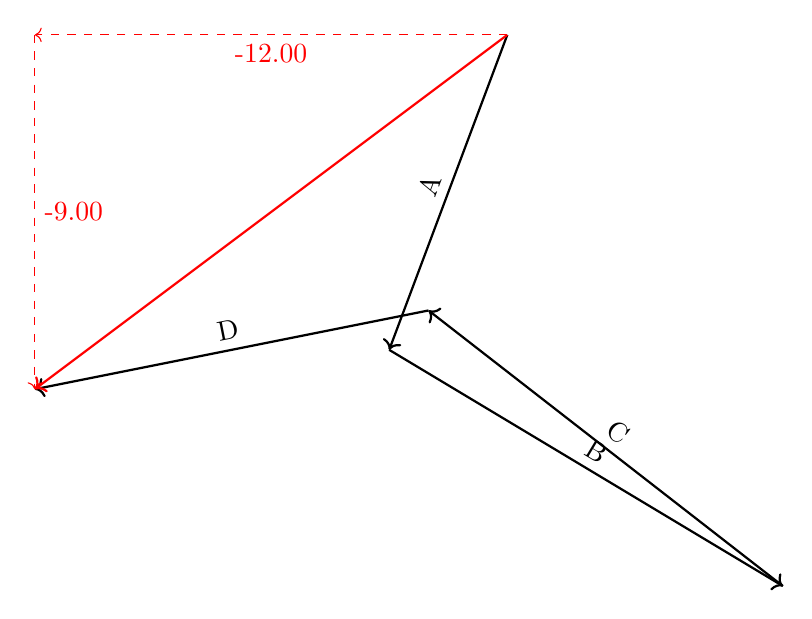
\begin{tikzpicture}[scale=0.5] 
\draw[->,black, thick] ( 0.00, 0.00) -- (-3.00,-8.00) node[midway,above,sloped]{ A } ;\draw[->,black, thick] (-3.00,-8.00) -- ( 7.00,-14.00) node[midway,above,sloped]{ B } ;\draw[->,black, thick] ( 7.00,-14.00) -- (-2.00,-7.00) node[midway,above,sloped]{ C } ;\draw[->,black, thick] (-2.00,-7.00) -- (-12.00,-9.00) node[midway,above,sloped]{ D } ;
\draw[->,red, thick] ( 0.00, 0.00) -- (-12.00,-9.00) node[midway,above,sloped]{  } ;
\draw[->,red,dashed] ( 0.00, 0.00) -- (-12.00, 0.00) node[midway,below]{ -12.00 };\draw[->,red,dashed] (-12.00, 0.00) -- (-12.00,-9.00) node[midway,right]{ -9.00 }; 
\end{tikzpicture} \\
\end{document}